\chapter{Método}
\label{cap:metodologia}

\section{Coleta de Dados}
\label{sec:col_dados}
Para este trabalho, será utilizada uma amostra de uma base de dados extraída do \gls{NPM}. Essa base contém informações sobre todos os pacotes hospedados no \gls{NPM} até jun/2017, totalizando \textit{366,629} pacotes. Para cada pacote, há informações sobre cada uma de suas \textit{releases}. A Tabela \ref{tab:database} contém as informações para o pacote \textit{buffer-includes}\footnote{https://npmjs.org/package/buffer-includes}, que contém os seguintes campos:

\begin{itemize}
    \item \textit{name}: o nome do pacote;
    \item \textit{version}: as versões de cada \textit{release} do pacote;
    \item \textit{timestamp}/\textit{prev\_timestamp}: contêm os \textit{timestamp} relacionados àquela determinada \textit{release};
    \item \textit{prov\_name}: os nomes dos provedores daquela \textit{release};
    \item \textit{prov\_vers}: contém, no momento da \textit{release} do cliente, a última versão dos provedores que o cliente aceitava; e
    \item \textit{prov\_chng}: informa o tipo de atualização que os provedores realizaram desde a última \textit{release} do cliente:
    \begin{itemize}
        \item se vazio: o provedor foi adicionado nesta \textit{release};
        \item \textit{steady}: a versão aceita do provedor não foi alterada desde a última \textit{release} do cliente, ou seja, o provedor não publicou nenhuma \textit{release} aceita pelo cliente; e
        \item \textit{upgrade}: após a última \textit{release} do cliente, o provedor publicou uma nova \textit{release} que o cliente aceita.
    \end{itemize}
\end{itemize}{}
  
\begin{table}[!h]
    \scalebox{0.72}{
        \begin{tabular}{|c|c|c|c|c|c|c|c|}
            \hline
            name & version & timestamp & prev\_timestamp & prov\_name & prov\_vers & prov\_chng \\ \hline
            buffer-includes & 0.1.0 & 2015-10-28T09:14:25.805Z &  & buf-indexof & 1.0.0 &  \\ \hline
            buffer-includes & 0.1.0 & 2015-10-28T09:14:25.805Z &  & ava & 0.3.0 &  \\ \hline
            buffer-includes & 0.1.0 & 2015-10-28T09:14:25.805Z &  & xo & 0.10.0 &  \\ \hline
            buffer-includes & 1.0.0 & 2016-09-30T08:23:30.480Z & 2015-10-28T09:14:25.805Z & buf-indexof & 1.0.0 & steady \\ \hline
            buffer-includes & 1.0.0 & 2016-09-30T08:23:30.480Z & 2015-10-28T09:14:25.805Z & ava & 1.0.0 & upgrade \\ \hline
            buffer-includes & 1.0.0 & 2016-09-30T08:23:30.480Z & 2015-10-28T09:14:25.805Z & xo & 0.16.0 & upgrade \\ \hline
        \end{tabular}
    }
    \caption{Formato da base de dados para cada pacote do NPM}
    \label{tab:database}
\end{table}

A base contém um total de \textit{366K} de projetos e por isso, realizar uma análise manual para um número gigantesco de projetos não é viável. Por isso, será utilizado uma amostra para o estudo de 384 pacotes, com base em um cálculo amostral\footnote{https://pt.surveymonkey.com/mp/sample-size-calculator/} com 95\% de confiança e 5\% de margem de erro. Dos \textit{366K} de pacotes, a amostra de 384 pacotes foi recuperada sorteando um número no intervalo \textit{0-366,629}. Do pacote sorteado, foi recuperado o seu \textit{package.json} e verificado se o pacote cumpre quatro requisitos: possui mais de 1 provedor --  se não houver provedores, não há possibilidades do pacote sofrer \textit{breaking changes}; possui um \textit{script} de teste não vazio e diferente do \textit{script} padrão de teste do \gls{NPM}: \textit{Error: no test specified}; possui a \textit{url} do repositório do pacote; e o repositório do pacote precisa existir -- será esperado de uma requisição \Gls{HTTP} para o repositório o código \textit{200} indicando sua existência. Todos esses requisitos foram analisados recuperando a \textit{release latest} do pacote, ou seja, a última \textit{release} disponível. A Figura \ref{fig:package_json} exemplifica as informações pertinentes no \textit{package.json} do pacote \textit{buffer-includes@1.0.0}\footnote{http://registry.npmjs.org/buffer-includes}.

\begin{figure}
    \centering
    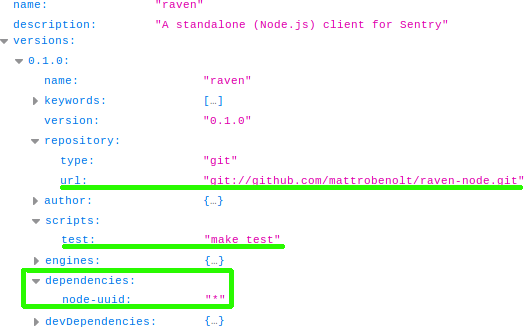
\includegraphics[scale=0.7]{figuras/package_json.png}
    \caption{Informações que serão recuperadas do \textit{package.json} para validar um pacote}
    \label{fig:package_json}
\end{figure}{}

Inicialmente, foram sorteados e executados 384 pacotes para o estudo, mas em 33 desses pacotes não foi possível executar o comando \textit{npm install}/\textit{npm test} para nenhuma de suas \textit{releases}. Isso porque esses pacotes apresentaram algum tipo de erro que impossibilitou a execução. Desses 33 pacotes, 15 não possuíam algum dos arquivos necessários para os testes; 10 continham \textit{scripts} de teste inválidos, tal como \textit{no tests}\footnote{https://github.com/djoulz22/drbd/blob/4920434f92656e6a49f09a56ef7eb4978ba6253c/package.json\#L7}; 4 haviam listados alguns dos arquivos no \textit{.gitignore} -- arquivo utilizado pelo \textit{git} para ignorar arquivos no repositório --, mas que eram necessários para a execução; 2 necessitaram de configurações específicas em banco de dados mas que não foi possível realizá-las; 1 pacote foi considerado como um \textit{toy package}, ou seja, não era um projeto real, apenas um repositório no qual o desenvolvedor, provavelmente, criou para testar o \gls{NPM}; e 1 pacote requeria uma variável de ambiente para acessar um determinado site. Então, os 33 pacotes foram substituídos em um novo sorteio seguindo o mesmo critério, totalizando 384 pacotes com 4544 \textit{releases} que foram utilizados no estudo. A Figura \ref{fig:database} apresenta a distribuição de provedores e de \textit{releases} entre a base e a amostra, na qual os \textit{boxplots} em azul -- dois primeiros -- representam a amostra e os \textit{boxplots} em vermelho -- dois últimos -- representam a base de dados.

\begin{figure}
    \centering
    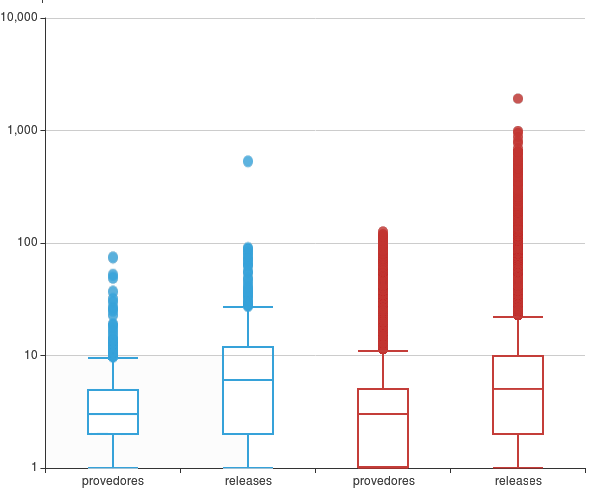
\includegraphics[scale=0.6]{figuras/data_box_plot_pt.png}
    \caption{Distribuição de provedores e \textit{releases} da amostra e da base, respectivamente}
    \label{fig:database}
\end{figure}{}

Em ambos os \textit{boxplots} da Figura \ref{fig:database}, o terceiro quartil e a mediana valem, respectivamente, 5 e 3 para os provedores. A maior discrepância visível nesta Figura é o quartil 1 entre os \textit{boxplots} dos provedores, uma vez que a quantidade de provedores, por pacote, abaixo da mediana representam 44\% para a amostra e 47\% para a base de dados, e esta discrepância aumenta conforme o número de provedores diminui. Já o terceiro quartil e a mediana dos \textit{boxplots} das \textit{releases} valem, respectivamente, 12 e 5 para a amostra e 10 e 5 para a base de dados. Por fim, o primeiro quartil vale 2 para ambos os \textit{boxplots} das \textit{releases}. Desta maneira, a amostra consegue representar suficientemente a base de dados.

Um detalhe importante se refere aos pacotes que utilizavam algum tipo de sistemas terceiros de banco de dados como o \textit{MySql\footnote{https://www.mysql.com}, Redis\footnote{https://redis.io}} entre outros sistemas. Então, quando um erro foi ocasionado pela falta de um destes sistemas, fez-se a habilitação e o pacote foi re-executado. Somente quando o pacote necessitava de uma configuração específica e que não foi possível configurá-la, então esse pacote foi substituído por outro.

\section{Ferramenta \textit{BCDetect} para executar os pacotes}
\label{sec:bcdetect}
Para executar os pacotes, foi desenvolvida uma ferramenta chamada \textit{BCDetect} disponível no \textit{GitHub}\footnote{https://github.com/danielventurini/bcdetect} sob a licença \textit{MIT}\footnote{https://choosealicense.com/licenses/mit}. Esta ferramenta recebe um arquivo de entrada no padrão da Tabela \ref{tab:database} e clona o repositório do respectivo pacote -- coincidentemente, todos os repositórios dos pacotes sorteados estavam hospedados no \textit{GitHub}. Após, é criado uma estrutura de dados para armazenar as informações extraídas do arquivo de entrada, na qual cada \textit{release} contém todas os provedores com suas versões e o tipo de atualização que os provedores realizaram desde a última \textit{release} do cliente. Esta estrutura está representada na Figura \ref{fig:bc_work}, que seria construída a partir da Tabela \ref{tab:database}.

\begin{figure}
    \centering
    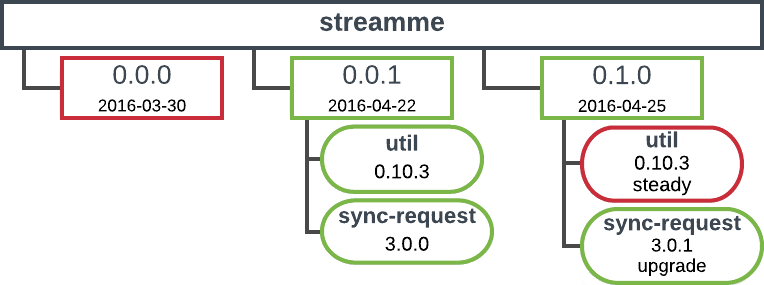
\includegraphics[scale=2]{figuras/bcdetect_work.png}
    \caption{Estrutura de dados para representar o arquivo de entrada da Tabela \ref{tab:database}}
    \label{fig:bc_work}
\end{figure}{}

Se uma \textit{release} houver provedores adicionados ou com novas versões aceitas -- \textit{upgrade} --, então essa \textit{release} é executada. Após clonado o repositório, é executado o comando \textit{git checkout} para restaurar a \textit{working tree} -- arquivos e sub-diretórios do repositório -- para a data da \textit{release} do cliente. Ao alterar a \textit{working tree}, todos os arquivos são restaurados para exatamente os mesmos arquivos do momento em que o cliente publicou a \textit{release}. Então o arquivo \textit{package-lock.json}\footnote{https://docs.npmjs.com/files/package-lock.json} é excluído -- se houver --, pois esse arquivo altera o comportamento do comando \textit{npm install} -- a partir do \textit{NPM@5} -- fazendo com que o \gls{NPM} instale as versões dos provedores de acordo com o \textit{package-lock.json}, e não de acordo com o \textit{package.json}. Após, é atualizado a versão dos provedores no campo \textit{dependencies} do \textit{package.json} para suas versões que foram recuperadas do arquivo. Esta operação não diferencia os provedores que estão no \textit{dependencies} ou no \textit{devDependencies}\footnote{além, há outros campos para dependências no \textit{package.json}, tais como o \textit{peerDependencies}, \textit{optionalDependencies} e o \textit{globalDependencies}}, uma vez que, para realizar o \textit{test}, ambos os provedores são requeridos. Por fim, é alterado a versão do \textit{Node.js} para a versão contida no campo \textit{engines\textrightarrow node} -- se houver -- no \textit{package.json} ou para a mais recente utilizando como referência a data da \textit{release} do cliente.

Para realizar a alteração da versão do \textit{Node.js} é utilizado como referência a data da \textit{release} do cliente. Através desta data, é possível identificar a última \textit{release} do \textit{Node.js} disponível\footnote{https://nodejs.org/en/download/releases} no momento da \textit{release} do cliente, ou seja, qual é a \textit{release} máxima do \textit{Node.js} que o cliente executou o pacote. Assim, o pacote é executado em todas as versões \textit{major} do \textit{Node.js}, da versão mais atual, pela data da \textit{release} do cliente, até a versão \textit{major} mais antiga. Para o pacote da Tabela \ref{tab:database}, a sua \textit{release 0.1.0} possui o \textit{timestamp 2016-04-25}, e a última \textit{release} do \textit{Node.js} disponível até esta data é a \textit{4.4.3}. Assim, este pacote foi executado com uma \textit{release 4.x, 3.x, 2.x, 1.x, 0.x} do \textit{Node.js}, até que uma dessas resultassem em sucesso na execução. Este chaveamento de versões do \textit{Node.js} é necessário pois um pacote que executa com sucesso na versão \textit{0.x} do \textit{Node.js}, por exemplo, provavelmente não irá executar com sucesso na versão \textit{8.x} do \textit{Node.js}. Desta forma, toda vez que a execução do pacote resulta em erro, é alterado a versão do \textit{Node.js} para a próxima \textit{release major} inferior e novamente é executado o pacote. Analogamente, esse problema de versões atinge o \gls{NPM}, mas ao alterar a versão do \textit{Node.js}, a versão do \gls{NPM} é atualizado também. Por fim, o \textit{BCDetect} salva as seguintes informações:

\begin{itemize}
    \item versão do pacote cliente;
    \item se houve alteração na versão aceita de alguns dos provedores;
    \item os códigos da execução do \textit{npm install} e \textit{npm test} -- sucesso ou erro;
    \item a versão do \textit{Node.js} que deveria ser executado com base na data da \textit{release}; e
    \item a versão do \textit{Node.js} que realmente o pacote executou com sucesso.
\end{itemize}{}

\section{Questões de Pesquisa}
\label{sec:qp}

\subsubsection{QP1. Com que frequência \textit{breaking changes} surgem \filipe{afetam? impactam?} nos pacotes clientes?}
\filipe{breaking change (defeito no provedor) vs. manifestação da breaking change (manifestação do defeito do provedor no cliente)}

No ecossistema do \gls{NPM} \filipe{npm em minúsculo}, uma \textit{release} que contenha um erro pode afetar uma grande quantidade de pacotes, uma vez que a rede de dependências do npm é relativamente densa \cite{teorical_reference:npm_2}. Para evitar que \textit{breaking changes} se manifestem nos pacotes clientes, os provedores introduzem as \textit{breaking changes} em \textit{releases major}, seguindo o padrão do Versionamento Semântico, e os cliente \filipe{clientes} podem utilizar \textit{strings semver} para aceitar apenas as versões \textit{minor} e \textit{patch} dos provedores -- o que é o padrão do \gls{NPM} \filipe{minúsculo}. Entretanto, nem sempre o provedor é capaz de distinguir se suas alterações são ou não \textit{breaking changes} \cite{noregrets2018}, ou, muitas vezes, as \textit{breaking changes} são introduzidas sem que o provedores percebam. Portanto, quando as \textit{breaking changes} são introduzidas em \textit{releases minor} ou \textit{patch}, elas podem causar comportamentos inesperados no cliente. Nesta RQ, será quantificado as manifestações das \textit{breaking changes} nos pacotes clientes. Assim, entender a frequência que os provedores publicam \textit{breaking changes} que afetam os clientes pode ajudar os clientes a fazer \filipe{tomar} decisões melhores sobre como e quando atualizar a versão do seu provedor.

\subsubsection{QP2. Como os pacotes provedores introduzem \textit{breaking changes} em uma \textit{release}?}

Pesquisas anteriores apresentam estudos sobre \textit{breaking changes} no ecossistema do \gls{NPM}. Entretanto, pelo fato do \textit{Javascript} ser dinâmico, estes estudos focaram apenas nas alterações de \gls{API}, tais como as remoções/renomeações, alterações na lista de parâmetros e alterações no tipo de retorno. Estes estudos foram realizados por  \citeonline{teorical_reference:bc_1} e \citeonline{noregrets2018} e não verificaram \textit{breaking changes} além das relacionadas às \gls{API}. Dessa maneira, além das alterações em \gls{API}, não se tem informações sobre como os provedores introduzem \textit{breaking changes}, ou seja, quais os principais casos que fazem com que o cliente sofra uma \textit{breaking changes}. Por causa da falta de informação, muitas \textit{breaking changes} são introduzidas, mas poderiam ser facilmente evitadas. Assim, grande parte das \textit{breaking changes} em \textit{JavaScript} são detectadas apenas em tempo de execução \cite{noregrets2018}, mas para o cliente, ter seu código encerrado em tempo de execução pode ser muito custoso. Por isso, dimensionar e categorizar as \textit{breaking changes} ajudará os desenvolvedores a atentar-se para as \textit{breaking changes} mais comuns e tentar evitá-las, assim produzindo códigos menos favoráveis às \textit{breaking changes}.

\subsubsection{QP3. Como os pacotes clientes se recuperam das \textit{breaking changes}?}

Uma vez que uma \textit{breaking changes} é introduzida, o cliente deve se recuperar dessa, ajustando o seu próprio código. Isso se faz necessário pois, no ecossistema do  \gls{NPM}, no qual centenas de milhares de pacotes estão conectados, uma simples \textit{release} com erro pode ocasionar na quebra de muitos clientes. No entanto, como os provedores evoluem independentemente dos clientes, erros e vulnerabilidades são difíceis de rastrear e corrigir nos clientes. Mesmo quando as vulnerabilidades podem ser corrigidas com a atualização para uma versão mais recente do provedor, pode haver incompatibilidades de \textit{API} -- entre outras incompatibilidades -- com os clientes que deve ser resolvido manualmente \cite{Foo:2018:ESC:3236024.3275535}. Dessa maneira, entender como os clientes reagem às \textit{breaking changes} ajudará os próprios clientes a conhecerem as alternativas frente às \textit{breaking changes} para que eles possam se recuperar da maneira mais eficiente.

\section{Cronograma de Atividades}
\label{cap:proposta:sec:cronograma}

Nesta seção são apresentadas as atividades a serem desenvolvidas para a execução da proposta. O cronograma de realização das tarefas é apresentado na Tabela~\ref{tab:cronograma}.

\begin{enumerate}
\item \textbf{Documentação da Ferramenta.}
\item \textbf{Obtenção dos dados da RQ3.}
\item \textbf{Análise dos Resultados.}
\item \textbf{Escrita do TCC 2.}
\item \textbf{Entrega do TCC 2.}
\item \textbf{Apresentação do TCC 2.}
\end{enumerate}

\begin{table}[h!]
\centering
\renewcommand{\arraystretch}{1.3}
\caption{Cronograma de atividades}
\label{tab:cronograma}
\scalefont{0.9}
\begin{tabular}{|c|c|c|c|c|c|}
\hline
\multirow{2}{*}{\textbf{Atividade}} & \multicolumn{2}{l|}{\textbf{2019}} & \multicolumn{3}{l|}{\textbf{2020}} \\ \cline{2-6} 
             & Nov & Dez & Jan & Fev & Mar \\ \hline
\textbf{1}   &  X  &     &     &     &     \\ \hline
\textbf{2}   &  X  &  X  &     &     &     \\ \hline
\textbf{3}   &  X  &  X  &     &     &     \\ \hline
\textbf{4}   &     &  X  &  X  &  X  &     \\ \hline
\textbf{5}   &     &     &     &     &  X  \\ \hline
\textbf{6}   &     &     &     &     &  X  \\ \hline
\end{tabular}
\end{table}